\section{Desarrollo}
A continuación se muestran los casos de uso encontrados para este aplicativo 
\begin{figure}[H]
	\hypertarget{fig:confi}{\hspace{1pt}}
	\begin{center}	
		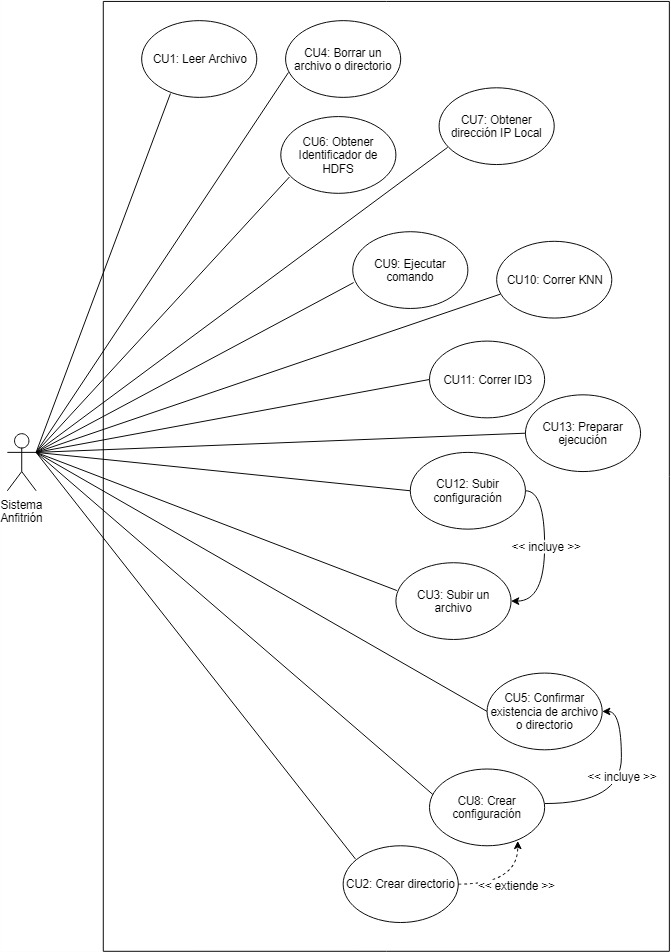
\includegraphics[width=.8\textwidth]{capitulo4a/images/diagramacu.jpeg}
		\caption{Diagrama de casos de uso}
		\label{fig:confi}
	\end{center}
\end{figure}
\begin{UseCase}{CU1}{Leer archivo}{

	Lee un archivo del sistema de archivos distribuidos a un stream especificado.

}

	\UCitem{Versión}{\color{Gray}0.1}

	\UCitem{Autor}{\color{Gray}Mayra Patricia Tovar Barba y Kevin Raúl Monteón Valdes.}

	\UCitem{Supervisa}{\color{Gray}Ulises Vélez Saldaña.}

	\UCitem{Actor}{Usuario Experto, Sistema.}

	\UCitem{Propósito}{Obtener un archivo del HDFS.}

	\UCitem{Entradas}{Ruta de archivo, Stream de salida, Identificador de HDFS, Dirección IP del Nodo Maestro.}

	\UCitem{Origen}{Teclado.}

	\UCitem{Salidas}{Ninguna.}

	\UCitem{Destino}{Stream de salida.}

	\UCitem{Precondiciones}{Debe existir el archivo de la ruta especificada.\newline El HDFS es accesible por la red.}

	\UCitem{Postcondiciones}{Los bytes del archivo habrán sido enviado a traves del stream de salida.}

	\UCitem{Errores}{LuminusException(1), IOException.}

	\UCitem{Tipo}{Caso de uso primario.}

	\UCitem{Observaciones}{}

\end{UseCase}

%--------------------------------------

\begin{UCtrayectoria}

	\UCpaso[\UCactor] Ocupa el método getDataFromFile.

	\UCpaso[\UCactor] Envía [{\em Ruta del Archivo}].

	\UCpaso[\UCactor] Envía [{\em Stream de Salida}].

	\UCpaso[\UCactor] Envía [{\em Identificador de HDFS}].

	\UCpaso[\UCactor] Envía [{\em Dirección IP del Nodo Maestro}].

	\UCpaso[\UCsist] Realiza una conexión al nodo maestro del HDFS por medio de la [{\em Dirección IP del Nodo Maestro}].\label{CU1conexion}

	\UCpaso[\UCsist] Verifica que la [{\em Ruta del Archivo}] exista. \refTray{A}

	\UCpaso[\UCsist] Copia en el [{\em Stream de Salida}] la información contenida en el archivo. \refTray{B}

	\UCpaso[\UCsist] Cierra la conexión al nodo maestro del HDFS creada en el paso \ref{CU1conexion}.

	\UCpaso[] Termina el caso de uso.

\end{UCtrayectoria}


%--------------------------------------		

	\begin{UCtrayectoriaA}{A}{Archivo no encontrado}

		\UCpaso Manda el Mensaje {\bf MSG1-}``La [{\em Ruta del Archivo}] no fue encontrada.''.

		\UCpaso[] Termina el caso de uso.

	\end{UCtrayectoriaA}

	

%--------------------------------------

	\begin{UCtrayectoriaA}{B}{Error al copiar}

		\UCpaso Manda el Mensaje con la información proporcionada por Java acerca del error de escritura o lectura.

		\UCpaso[] Termina el caso de uso.

	\end{UCtrayectoriaA}



%%%%%%%%%%%%%%%%%%%%%%%%%%%%%%%%%%%%%%%%%%%%%%%%%%%%%%%%%%%%%%%%

\begin{UseCase}{CU2}{Crear directorio}{

Crea un directorio en el sistema de archivos distribuidos.

}

\UCitem{Versión}{\color{Gray}0.1}

\UCitem{Autor}{\color{Gray}Mayra Patricia Tovar Barba y Kevin Raúl Monteón Valdes}

\UCitem{Supervisa}{\color{Gray}Ulises Vélez Saldaña.}

\UCitem{Actor}{Usuario Experto, Sistema.}

\UCitem{Propósito}{Crear un directorio en el HDFS.}

\UCitem{Entradas}{Ruta de directorio, Identificador de HDFS, Dirección IP del Nodo Maestro.}

\UCitem{Origen}{Teclado.}

\UCitem{Salidas}{Ninguna.}

\UCitem{Destino}{Ninguno.}

\UCitem{Precondiciones}{No debe existir el directorio en la [{\em Ruta del directorio}] especificada.\newline El HDFS es accesible por la red.}

\UCitem{Postcondiciones}{Se crea un nuevo directorio en la [{\em Ruta del directorio}] especificada.}

\UCitem{Errores}{LuminusException(3).}

\UCitem{Tipo}{Caso de uso primario.}

\UCitem{Observaciones}{}

\end{UseCase}

%--------------------------------------

\begin{UCtrayectoria}

\UCpaso[\UCactor] Ocupa el método makeHDFSDirectory

\UCpaso[\UCactor] Envía [{\em Ruta de directorio}].

\UCpaso[\UCactor] Envía [{\em Identificador de HDFS}].

\UCpaso[\UCactor] Envía [{\em Dirección IP del Nodo Maestro}].

\UCpaso[\UCsist] Realiza una conexión al nodo maestro del HDFS por medio del [{\em Identificador de HDFS}]\label{CU2conexion}

\UCpaso[\UCsist] Verifica que la [{\em Ruta del directorio}] no exista \refTray{A}

\UCpaso[\UCsist] Crea un nuevo directorio en la [{\em Ruta del directorio}] especificada.

\UCpaso[\UCsist] Cierra la conexión al nodo maestro del HDFS creada en el paso \ref{CU2conexion}

\UCpaso[] Termina el caso de uso.

\end{UCtrayectoria}



%--------------------------------------		

\begin{UCtrayectoriaA}{A}{Directorio ya existe}

	\UCpaso Manda el Mensaje {\bf MSG1-}``La [{\em Ruta del directorio}] ya existe.''.

	\UCpaso[] Termina el caso de uso.

\end{UCtrayectoriaA}



%%%%%%%%%%%%%%%%%%%%%%%%%%%%%%%%%%%%%%%%%%%%%%%%%%%%%%%%%%%%%%%%

\begin{UseCase}{CU3}{Subir un archivo}{

Almacena información a un archivo del sistema de archivos distribuidos.

}

\UCitem{Versión}{\color{Gray}0.1}

\UCitem{Autor}{\color{Gray}Mayra Patricia Tovar Barba y Kevin Raúl Monteón Valdes}

\UCitem{Supervisa}{\color{Gray}Ulises Vélez Saldaña.}

\UCitem{Actor}{Usuario Experto, Sistema.}

\UCitem{Propósito}{Sube un archivo al HDFS.}

\UCitem{Entradas}{Ruta de archivo local, Ruta de archivo remoto, Identificador de HDFS, Bandera de Sobrescribir.}

\UCitem{Origen}{Teclado.}

\UCitem{Salidas}{Ninguna.}

\UCitem{Destino}{Ninguno.}

\UCitem{Precondiciones}{El HDFS es accesible por la red.}

\UCitem{Postcondiciones}{Se crea o actualiza un archivo en la [{\em Ruta de archivo remoto}] especificada.}

\UCitem{Errores}{Ninguno.}

\UCitem{Tipo}{Caso de uso primario.}

\UCitem{Observaciones}{}

\end{UseCase}

%--------------------------------------

\begin{UCtrayectoria}

\UCpaso[\UCactor] Ocupa el método uploadFileToHDFS

\UCpaso[\UCactor] Envía [{\em Ruta de archivo local}].

\UCpaso[\UCactor] Envía [{\em Ruta de archivo remoto}].

\UCpaso[\UCactor] Envía [{\em Identificador de HDFS}].

\UCpaso[\UCactor] Envía [{\em Bandera de Sobrescribir}].

\UCpaso[\UCsist] Realiza una conexión al nodo maestro del HDFS por medio del [{\em Identificador de HDFS}].\label{CU3conexion}

\UCpaso[\UCsist] Verifica que el archivo en la [{\em Ruta de archivo remoto}] no exista. \refTray{A} \refTray{B}

\UCpaso[\UCsist] Copia el archivo local de la [{\em Ruta de archivo local}] al archivo remoto de la [{\em Ruta de archivo remoto}].\label{copia}

\UCpaso[\UCsist] Cierra la conexión al nodo maestro del HDFS creada en el paso \ref{CU3conexion}.

\UCpaso[] Termina el caso de uso.

\end{UCtrayectoria}



%--------------------------------------		

\begin{UCtrayectoriaA}{A}{Sobrescribir archivo}

	\UCpaso Verifica que la [{\em Bandera de Sobrescribir}] esta activada.

	\UCpaso[] Reanuda el caso de uso \refUC{CU3} en el paso \ref{copia}.

\end{UCtrayectoriaA}



\begin{UCtrayectoriaA}{B}{No sobrescribir archivo}

	\UCpaso Verifica que la [{\em Bandera de Sobrescribir}] esta desactivada.

	\UCpaso Manda el Mensaje {\bf MSG1-}``El archivo remoto ya existe.''.

	\UCpaso[] Termina el caso de uso.

\end{UCtrayectoriaA}



%%%%%%%%%%%%%%%%%%%%%%%%%%%%%%%%%%%%%%%%%%%%%%%%%%%%%%%%%%%%%%%%

\begin{UseCase}{CU4}{Borrar un archivo o directorio}{

Elimina un archivo o directorio del sistema de archivos distribuidos.

}

\UCitem{Versión}{\color{Gray}0.1}

\UCitem{Autor}{\color{Gray}Mayra Patricia Tovar Barba y Kevin Raúl Monteón Valdes}

\UCitem{Supervisa}{\color{Gray}Ulises Vélez Saldaña.}

\UCitem{Actor}{Usuario Experto, Sistema.}

\UCitem{Propósito}{Elimina un archivo o directorio del HDFS.}

\UCitem{Entradas}{Ruta de archivo o directorio, Identificador de HDFS}

\UCitem{Origen}{Teclado.}

\UCitem{Salidas}{Ninguna.}

\UCitem{Destino}{Ninguno.}

\UCitem{Precondiciones}{El archivo o directorio en la [{\em Ruta de archivo o directorio}] debe existir en el HDFS.\newline El HDFS es accesible por la red.}

\UCitem{Postcondiciones}{Se elimina el archivo o directorio en la [{\em Ruta de archivo o directorio}].}

\UCitem{Errores}{LuminusException(1).}

\UCitem{Tipo}{Caso de uso primario.}

\UCitem{Observaciones}{}

\end{UseCase}

%--------------------------------------

\begin{UCtrayectoria}

\UCpaso[\UCactor] Ocupa el método deleteFromHDFS

\UCpaso[\UCactor] Envía [{\em Ruta de archivo o directorio}].

\UCpaso[\UCactor] Envía [{\em Identificador de HDFS}].

\UCpaso[\UCsist] Realiza una conexión al nodo maestro del HDFS por medio del [{\em Identificador de HDFS}]\label{CU4conexion}

\UCpaso[\UCsist] Verifica que el archivo o directorio en la[{\em Ruta de archivo o directorio}] exista. \refTray{A}

\UCpaso[\UCsist] Elimina el archivo o directorio de la [{\em Ruta de archivo o directorio}].

\UCpaso[\UCsist] Cierra la conexión al nodo maestro del HDFS creada en el paso \ref{CU4conexion}.

\UCpaso[] Termina el caso de uso.

\end{UCtrayectoria}



%--------------------------------------		

\begin{UCtrayectoriaA}{A}{No existe el archivo o directorio}

	\UCpaso Manda el Mensaje {\bf MSG1-}``El archivo o directorio en la [{\em Ruta de archivo o directorio}] no existe.''.

	\UCpaso[] Termina el caso de uso.

\end{UCtrayectoriaA}



%%%%%%%%%%%%%%%%%%%%%%%%%%%%%%%%%%%%%%%%%%%%%%%%%%%%%%%%%%%%%%%%

\begin{UseCase}{CU5}{Confirmar existencia de archivo o directorio}{

Confirma la existencia de un archivo o un directorio en un sistema de archivos distribuidos

}

\UCitem{Versión}{\color{Gray}0.1}

\UCitem{Autor}{\color{Gray}Mayra Patricia Tovar Barba y Kevin Raúl Monteón Valdes}

\UCitem{Supervisa}{\color{Gray}Ulises Vélez Saldaña.}

\UCitem{Actor}{Usuario Experto, Sistema.}

\UCitem{Propósito}{Confirma la existencia de un archivo o directorio.}

\UCitem{Entradas}{Ruta de archivo o directorio, Identificador de HDFS}

\UCitem{Origen}{Teclado.}

\UCitem{Salidas}{Existe, No Existe}

\UCitem{Destino}{Ninguno.}

\UCitem{Precondiciones}{El HDFS es accesible por la red.}

\UCitem{Postcondiciones}{Se confirmo si el archivo o directorio en la [{\em Ruta de archivo o directorio}] existe.}

\UCitem{Errores}{IllegalArgumentException, IOException.}

\UCitem{Tipo}{Caso de uso primario.}

\UCitem{Observaciones}{}

\end{UseCase}

%--------------------------------------

\begin{UCtrayectoria}

\UCpaso[\UCactor] Ocupa el método existsInHDFS

\UCpaso[\UCactor] Envía [{\em Ruta de archivo o directorio}].

\UCpaso[\UCactor] Envía [{\em Identificador de HDFS}].

\UCpaso[\UCsist] Realiza una conexión al nodo maestro del HDFS por medio del [{\em Identificador de HDFS}]\label{CU5conexion}

\UCpaso[\UCsist] Consulta al archivo o directorio en la[{\em Ruta de archivo o directorio}]. \refTray{A} \refTray{B}

\end{UCtrayectoria}



%--------------------------------------		

\begin{UCtrayectoriaA}{A}{No existe el archivo o directorio}

	\UCpaso Manda el Mensaje {\bf MSG1-}``El archivo o directorio en la [{\em Ruta de archivo o directorio}] no existe.''.

	\UCpaso[\UCsist] Cierra la conexión al nodo maestro del HDFS creada en el paso \ref{CU5conexion}.

	\UCpaso[\UCsist] Retorna el valor "No Existe"

	\UCpaso[] Termina el caso de uso.

\end{UCtrayectoriaA}



\begin{UCtrayectoriaA}{A}{Existe el archivo o directorio}

	\UCpaso Manda el Mensaje {\bf MSG1-}``El archivo o directorio en la [{\em Ruta de archivo o directorio}] existe.''.

	\UCpaso[\UCsist] Cierra la conexión al nodo maestro del HDFS creada en el paso \ref{CU5conexion}.

	\UCpaso[\UCsist] Retorna el valor "Existe"

	\UCpaso[] Termina el caso de uso.

\end{UCtrayectoriaA}



%%%%%%%%%%%%%%%%%%%%%%%%%%%%%%%%%%%%%%%%%%%%%%%%%%%%%%%%%%%%%%%%

\begin{UseCase}{CU6}{Obtener Identificador de HDFS}{

Obtiene el Identificador de HDFS a partir de una Dirección IP de Nodo Maestro.

}

\UCitem{Versión}{\color{Gray}0.1}

\UCitem{Autor}{\color{Gray}Mayra Patricia Tovar Barba y Kevin Raúl Monteón Valdes}

\UCitem{Supervisa}{\color{Gray}Ulises Vélez Saldaña.}

\UCitem{Actor}{Usuario Experto, Sistema.}

\UCitem{Propósito}{Recupera el Identificador de HDFS.}

\UCitem{Entradas}{Dirección IP de Nodo Maestro.}

\UCitem{Origen}{Teclado.}

\UCitem{Salidas}{Ninguna.}

\UCitem{Destino}{Ninguno.}

\UCitem{Precondiciones}{El nodo maestro es accesible por la red.}

\UCitem{Postcondiciones}{Se elimina el archivo o directorio en la [{\em Ruta de archivo o directorio}].}

\UCitem{Errores}{IOException.}

\UCitem{Tipo}{Caso de uso primario.}

\UCitem{Observaciones}{}

\end{UseCase}

%--------------------------------------

\begin{UCtrayectoria}

\UCpaso[\UCactor] Ocupa el método deleteFromHDFS

\UCpaso[\UCactor] Envía [{\em Ruta de archivo o directorio}].

\UCpaso[\UCactor] Envía [{\em Identificador de HDFS}].

\UCpaso[\UCsist] Realiza una conexión al nodo maestro del HDFS por medio del [{\em Identificador de HDFS}]\label{CU6conexion}

\UCpaso[\UCsist] Verifica que el archivo o directorio en la[{\em Ruta de archivo o directorio}] exista. \refTray{A}

\UCpaso[\UCsist] Elimina el archivo o directorio de la [{\em Ruta de archivo o directorio}].

\UCpaso[\UCsist] Cierra la conexión al nodo maestro del HDFS creada en el paso \ref{CU6conexion}.

\UCpaso[] Termina el caso de uso.

\end{UCtrayectoria}



%--------------------------------------		

\begin{UCtrayectoriaA}{A}{No existe el archivo o directorio}

	\UCpaso Manda el Mensaje {\bf MSG1-}``El archivo o directorio en la [{\em Ruta de archivo o directorio}] no existe.''.

	\UCpaso[] Termina el caso de uso.

\end{UCtrayectoriaA}



%%%%%%%%%%%%%%%%%%%%%%%%%%%%%%%%%%%%%%%%%%%%%%%%%%%%%%%%%%%%%%%%

\begin{UseCase}{CU7}{Obtener Dirección IP Local}{

Obtiene la Dirección IP Local asignada a la interfaz de red por defecto.

}

\UCitem{Versión}{\color{Gray}0.1}

\UCitem{Autor}{\color{Gray}Mayra Patricia Tovar Barba y Kevin Raúl Monteón Valdes}

\UCitem{Supervisa}{\color{Gray}Ulises Vélez Saldaña.}

\UCitem{Actor}{Usuario Experto, Sistema.}

\UCitem{Propósito}{Recupera la Dirección IP Local.}

\UCitem{Entradas}{Ninguna.}

\UCitem{Origen}{Teclado.}

\UCitem{Salidas}{Cadena conteniendo [{\em Dirección IP Local}].}

\UCitem{Destino}{Ninguno.}

\UCitem{Precondiciones}{Ninguna.}

\UCitem{Postcondiciones}{Se conoce la [{\em Dirección IP Local}].}

\UCitem{Errores}{UnknownHostException.}

\UCitem{Tipo}{Caso de uso primario.}

\UCitem{Observaciones}{}

\end{UseCase}

%--------------------------------------

\begin{UCtrayectoria}

\UCpaso[\UCactor] Ocupa el método getLocalNetAddress

\UCpaso[\UCsist] Recupera la [{\em Dirección IP Local}] \refTray{A}

\UCpaso[\UCsist] Retorna una cadena con el valor de la [{\em Dirección IP Local}]

\UCpaso[] Termina el caso de uso.

\end{UCtrayectoria}



%--------------------------------------		

\begin{UCtrayectoriaA}{A}{Error al Recuperar Dirección IP Local}

	\UCpaso Manda el Mensaje con la información proporcionada por Java acerca del error de recuperación de la [{\em Dirección IP Local}]

	\UCpaso[] Termina el caso de uso.

\end{UCtrayectoriaA}

%%%%%%%%%%%%%%%%%%%%%%%%%%%%%%%%%%%%%%%%%%%%%%%%%%%%%%%%%%%%%%%%

\begin{UseCase}{CU8}{Crear configuración}{

		Crea un objeto de configuración cuyas propiedades son guardados en sistema de archivos local

	}

		\UCitem{Versión}{\color{Gray}0.1}

		\UCitem{Autor}{\color{Gray}Mayra Patricia Tovar Barba y Kevin Raúl Monteón Valdes}

		\UCitem{Supervisa}{\color{Gray}Ulises Vélez Saldaña.}

		\UCitem{Actor}{Usuario Experto, Sistema.}

		\UCitem{Propósito}{Generar un objeto de configuración.}

		\UCitem{Entradas}{Ninguna.}

		\UCitem{Origen}{Teclado.}

		\UCitem{Salidas}{Propiedades de objeto de configuración.}

		\UCitem{Destino}{Sistema de archivos local.}

		\UCitem{Precondiciones}{Ninguna.}

		\UCitem{Postcondiciones}{Las propiedades del archivo de configuracion generados son escritas al sistema de archivos local.}

		\UCitem{Errores}{IOException.}

		\UCitem{Tipo}{Caso de uso primario.}

		\UCitem{Observaciones}{}

	\end{UseCase}

%--------------------------------------

	\begin{UCtrayectoria}

		\UCpaso[\UCactor] Ocupa el método createConfiguration.

		\UCpaso[\UCsist] Crea el archivo "configuration.properties" localmente y genera su contenido basado en variables previamente definidas.

		\UCpaso[\UCsist] Se invoca al caso de uso \refUC{CU5}{Confirmar existencia de archivo o directorio}

		\UCpaso[\UCsist] Se valida la existencia del directorio que alojara el archivo de configuración en el HDFS \refTray{A}

		\UCpaso[] Termina el caso de uso.

	\end{UCtrayectoria}



%--------------------------------------		

	\begin{UCtrayectoriaA}{A}{Directorio no existe}

		\UCpaso[\UCsist] Se invoca al caso de uso \refUC{CU2}{Crear directorio}

		\UCpaso[] Termina el caso de uso.

	\end{UCtrayectoriaA}

%%%%%%%%%%%%%%%%%%%%%%%%%%%%%%%%%%%%%%%%%%%%%%%%%%%%%%%%%%%%%%%%

	\begin{UseCase}{CU9}{Ejecutar Comando}{

		Envia comando al runtime para ser ejecutado

	}

		\UCitem{Versión}{\color{Gray}0.1}

		\UCitem{Autor}{\color{Gray}Mayra Patricia Tovar Barba y Kevin Raúl Monteón Valdes}

		\UCitem{Supervisa}{\color{Gray}Ulises Vélez Saldaña.}

		\UCitem{Actor}{Usuario Experto, Sistema.}

		\UCitem{Propósito}{Enviar comando a proceso en ejecucion.}

		\UCitem{Entradas}{Comando.}

		\UCitem{Origen}{Teclado.}

		\UCitem{Salidas}{De acuerdo a comando.}

		\UCitem{Destino}{Proceso en ejecución.}

		\UCitem{Precondiciones}{Debe existir el proceso.}

		\UCitem{Postcondiciones}{El proceso recibe el comando y lo ejecuta apropiadamente.}

		\UCitem{Errores}{IOException.}

		\UCitem{Tipo}{Caso de uso primario.}

		\UCitem{Observaciones}{}

	\end{UseCase}

	%--------------------------------------

	\begin{UCtrayectoria}

		\UCpaso[\UCactor] Ocupa el método executeCommand.

		\UCpaso[\UCsist] Obtiene la instancia del proceso en ejecución.

		\UCpaso[\UCsist] Utiliza el método del proceso para comunicación de comandos.

		\UCpaso[\UCsist] Muestra salida del comando si hay alguna.

		\UCpaso[\UCsist] Muestra errores del comando si hay alguno.

		\UCpaso[] Termina el caso de uso.

	\end{UCtrayectoria}



	%%%%%%%%%%%%%%%%%%%%%%%%%%%%%%%%%%%%%%%%%%%%%%%%%%%%%%%%%%%%%%%%

	\begin{UseCase}{CU10}{Correr KNN}{

		Pasa parametros a la clase de LuminusKNN para su ejecucion.

	}

		\UCitem{Versión}{\color{Gray}0.1}

		\UCitem{Autor}{\color{Gray}Mayra Patricia Tovar Barba y Kevin Raúl Monteón Valdes}

		\UCitem{Supervisa}{\color{Gray}Ulises Vélez Saldaña.}

		\UCitem{Actor}{Usuario Experto, Sistema.}

		\UCitem{Propósito}{Ejecutar algoritmo de KNN.}

		\UCitem{Entradas}{Ninguna.}

		\UCitem{Origen}{Teclado.}

		\UCitem{Salidas}{Archivo de resultados de KNN}

		\UCitem{Destino}{Sistema de archivos distribuidos.}

		\UCitem{Precondiciones}{Debe existir una configuración valida en el HDFS.}

		\UCitem{Postcondiciones}{Se genera un archivo con los resultados de la ejecución en el HDFS.}

		\UCitem{Errores}{Ninguno.}

		\UCitem{Tipo}{Caso de uso primario.}

		\UCitem{Observaciones}{}

	\end{UseCase}

	%--------------------------------------

	\begin{UCtrayectoria}

		\UCpaso[\UCactor] Ocupa el método runKNN.

		\UCpaso[\UCsist] Crea una cadena de parámetros a ser pasados a la clase LuminusKNN

		\UCpaso[\UCsist] Se invoca a la clase LuminusKNN con los parámetros especificados.

		\UCpaso[] Termina el caso de uso.

	\end{UCtrayectoria}



		%%%%%%%%%%%%%%%%%%%%%%%%%%%%%%%%%%%%%%%%%%%%%%%%%%%%%%%%%%%%%%%%

	\begin{UseCase}{CU10}{Correr ID3}{

		Pasa parámetros a la clase de LuminusKNN para su ejecución.

	}

		\UCitem{Versión}{\color{Gray}0.1}

		\UCitem{Autor}{\color{Gray}Mayra Patricia Tovar Barba y Kevin Raúl Monteón Valdes}

		\UCitem{Supervisa}{\color{Gray}Ulises Vélez Saldaña.}

		\UCitem{Actor}{Usuario Experto, Sistema.}

		\UCitem{Propósito}{Ejecutar algoritmo de ID3.}

		\UCitem{Entradas}{Ninguna.}

		\UCitem{Origen}{Teclado.}

		\UCitem{Salidas}{Archivo de resultados de ID3}

		\UCitem{Destino}{Sistema de archivos distribuidos.}

		\UCitem{Precondiciones}{Debe existir una configuración valida en el HDFS.}

		\UCitem{Postcondiciones}{Se genera un archivo con los resultados de la ejecución en el HDFS.}

		\UCitem{Errores}{Ninguno.}

		\UCitem{Tipo}{Caso de uso primario.}

		\UCitem{Observaciones}{}

	\end{UseCase}

	%--------------------------------------

	\begin{UCtrayectoria}

		\UCpaso[\UCactor] Ocupa el método runID3.

		\UCpaso[\UCsist] Crea una cadena de parámetros a ser pasados a la clase LuminusID3.

		\UCpaso[\UCsist] Se invoca a la clase LuminusKNN con los parámetros especificados.

		\UCpaso[] Termina el caso de uso.

	\end{UCtrayectoria}

	%%%%%%%%%%%%%%%%%%%%%%%%%%%%%%%%%%%%%%%%%%%%%%%%%%%%%%%%%%%%%%%%

	\begin{UseCase}{CU12}{Subir Configuración}{

		Sube el archivo de configuración generado localmente al sistema de archivos distribuidos.

	}

		\UCitem{Versión}{\color{Gray}0.1}

		\UCitem{Autor}{\color{Gray}Mayra Patricia Tovar Barba y Kevin Raúl Monteón Valdes}

		\UCitem{Supervisa}{\color{Gray}Ulises Vélez Saldaña.}

		\UCitem{Actor}{Usuario Experto, Sistema.}

		\UCitem{Propósito}{Subir configuración a HDFS.}

		\UCitem{Entradas}{Ninguna.}

		\UCitem{Origen}{Teclado.}

		\UCitem{Salidas}{Ninguna.}

		\UCitem{Destino}{Sistema de archivos distribuidos.}

		\UCitem{Precondiciones}{Ninguna.}

		\UCitem{Postcondiciones}{Se encuentra una copia del archivo de configuración en el sistema de archivos distribuidos.}

		\UCitem{Errores}{IOException.}

		\UCitem{Tipo}{Caso de uso primario.}

		\UCitem{Observaciones}{}

	\end{UseCase}

	%--------------------------------------

	\begin{UCtrayectoria}

		\UCpaso[\UCactor] Ocupa el método uploadConfigurations.

		\UCpaso[\UCsist] Invoca al método \refUC{CU3}{Subir un archivo} con argumentos del archivo de configuración.

		\UCpaso[] Termina el caso de uso.

	\end{UCtrayectoria}

	%%%%%%%%%%%%%%%%%%%%%%%%%%%%%%%%%%%%%%%%%%%%%%%%%%%%%%%%%%%%%%%%

	\begin{UseCase}{CU13}{Preparar Ejecución}{

		Crea un objeto de configuración cuyas propiedades son guardados en sistema de archivos local

	}

		\UCitem{Versión}{\color{Gray}0.1}

		\UCitem{Autor}{\color{Gray}Mayra Patricia Tovar Barba y Kevin Raúl Monteón Valdes}

		\UCitem{Supervisa}{\color{Gray}Ulises Vélez Saldaña.}

		\UCitem{Actor}{Usuario Experto, Sistema.}

		\UCitem{Propósito}{Validar el objeto de configuración.}

		\UCitem{Entradas}{Ninguna.}

		\UCitem{Origen}{Teclado.}

		\UCitem{Salidas}{Valido o Invalido.}

		\UCitem{Destino}{Pantalla.}

		\UCitem{Precondiciones}{Ninguna.}

		\UCitem{Postcondiciones}{Se conoce la valides del archivo de configuración.}

		\UCitem{Errores}{IOException.}

		\UCitem{Tipo}{Caso de uso primario.}

		\UCitem{Observaciones}{}

	\end{UseCase}

	%--------------------------------------

	\begin{UCtrayectoria}

		\UCpaso[\UCactor] Ocupa el método isReadyToExecute.

		\UCpaso[\UCsist] Lee el archivo "configuration.properties" localmente

		\UCpaso[\UCsist] Valida que todas las propiedades necesarias sean correctas \refTray{A}

		\UCpaso[\UCsist] Retorna el valor "Valido"

		\UCpaso[] Termina el caso de uso.

	\end{UCtrayectoria}



	%--------------------------------------		

	\begin{UCtrayectoriaA}{A}{Falta una configuración}

		\UCpaso[\UCsist] Retorna el valor "Invalido"

		\UCpaso[] Termina el caso de uso.

	\end{UCtrayectoriaA}
